\documentclass{article}
\bibliographystyle{plain}
\usepackage{tikz}
\usepackage{bibentry}
\usepackage{multicol}
\usepackage{enumitem}
\usepackage{blindtext}
\usepackage{graphicx}
\usepackage{amsmath, amssymb}
\usepackage[margin=1in]{geometry}
\setlength{\parindent}{2em}
\begin{document}
\title{CMPS 278 Final}
\author{Austen Barker}
\maketitle

%\begin{multicols}{1}

\textbf{Abstract:} 
Parallelization is becoming more common in database technology and there is little being done in the area of log rollback. With parallelization it is possible to obtain small but important performance gains when applying logs to a database or enable a database administrator to roll back to a previous instance at will. So long as the log possess the requisite detail. This paper explores the viability of a parallelized database log application system that breaks up the log into discrete chunks and computes summaries that can then be applied to the database. Such a system is implemented and used to demonstrate the possible performance and flexibility to be gained from using such a log application technique.

\section{Introduction}
With the movement towards more multicore parallelizable workloads in database systems it is worth wondering whether or not it is worth while to give the same treatment to how logs are handled. Many modern database systems utilize some form of logging in order to provide ACID characteristics for their transactions, backup, and recovery features. Through systems such as Write Ahead Logging, undo operations done with the support of a database transaction log are relatively common\cite{WAL}. Although what is not explored is the ability to reapply these logs as undo operations in parallel by breaking up the log to be rolled back into discrete chunks. These discrete chunks could then be applied to the database in batches as either part of the undo step of a recovery algorithm or in order to restore the state of the database to some desired previous point in time at the user's behest.

This paper presents a database logging system built on top of the BerkeleyDB key/value store that provides sufficient detail in its logging records to enable reconstruction of a database at any point in time that is described by the log. This is accomplished through compositing operations described in the log into a summary of all changes to the database between two points in time or log sequence numbers. One or more of these summaries are then applied to the database in order to produce an instance of the database as it existed at a previous time.
\section{Problem}
The problem posed is whether or not it is feasible or worthwhile to parallelize log roll back, undo, redo, etc by computing summaries of discrete chunks of log records that can then each be applied to a database to reconstruct its state at a previous time.

\subsection{Background} 
Among current database systems there are very few that enable a roll back to a specific time stamp that can be invoked by the user or that is executed in parallel. Most simply utilize their logging infrastructure to ensure basic ACID characteristics or for backup and recovery tasks and are executed linearly.

In the case of Databases such as PostgreSQL and the InnoDB component of MySQL will utilize their write ahead log not only for redo and undo operations similarly to write ahead logging but they will also use them for backup operations and something called point-in-time recovery (PITR)\cite{InnoDBpoint} \cite{Postgrespoint}. PITR enables a full backup of the database to be stored at regular intervals and then be restored to the latest state of the database by playing redo operations from the log on top of the backup.

Very similar in theory to what we wished to accomplish is the concept of a 'rollback segment' as seen in InnoDB \cite{InnoDBredo}. Although these rollback segments in actuality are data structures that are used to organize the transaction logs into easily manageable pieces as opposed to processed summaries.

Many write ahead logging implementations do not store there logs for long. In the case of databases like SQLite and InnoDB there is a limit to either how much storage is used to contain the log or how old log records are permitted to be. In the case of SQLite we see that log records are stored in temporary files and are disposed of at either regular time intervals or when all active sessions with the database are closed \cite{SQLiteLog}. In the case of InnoDB we see that there is a limited number of log segments that can store the logs needed to rollback the database\cite{InnoDBUndo}.


\section{Project}
The overarching aim of this project was to explore the viability of performing log application methods in parallel by computing summaries of discrete sections of the log and applying these summaries to the database. To explore this concept a testing system was to be built as a proof-of-concept and to return quantitative results on whether or not the system provides any performance advantages over applying the log to the database in order. A set of three milestones were established in order to break the project up into manageable stages that would build on one another. 

\subsection{Goals}
The overall goal of this project was to produce a piece of software that could roll up discrete chunks
of the log. Then use these chunks in order to reconstruct the state of the database at any time that
the log covered. The available period of time available for a roll up would depend on the implementation
of the database's logging system. Chunks could be computed in parallel, depending on the locking scheme
used by the logging system in question. Three major milestones were set in place on the project's roadmap.\\

\textbf{A)} The first milestone would be a basic application that could take the log provided by a database
and process the discrete chunks of the database based on a timestamp or log sequence number (LSN). This was 
the "proof of concept" step to show whether or not the idea could work. This would then be compared to some
existing logging and recovery methods such as write-ahead logging.\\

\textbf{B)} The second milestone involves storing specific save points to the disk that would contain what 
is essentially a "diff" of the database between the start and end of a log chunk. This diff would be 
analogous to the output of the unix command "diff". Also included in this milestone is parallelized execution.
Though that would depend on whether or not the system was implemented in a lower level language such as C/C++. This step would be the minimum for producing results if the system was implemented in a lower level language.\\

\textbf{C)} The final milestone and coup de grace of the project would be its inclusion into an existing
database system or the implementation of a new one. Most likely this would manifest itself in a simpler
relational database such as SQLite. Primarily due to the small size of the source code.\\

In the end a smattering of the three different milestones manifested themselves in the final implementation. It contained the objective of the first milestone, the parallelized element of the second and the interface with an existing database system from the third.\\

\subsection{SQLite background}
Initially the logs used for the testing of whatever form the new implementation would take were to come from a small instance of PostgreSQL. Although it became clear from the lack of easily located documentation concerning its logging infrastructure that it would not be practical to use for the initial proof of concept. This led to a transition to SQLite. A small and lightweight relational database intended for use in embedded applications such as is commonly found in web applications. A small python application was used to randomly insert, update, retrieve, and delete records in a single table at regular intervals.
 
SQLite has two major logging methods. Either write-ahead logging or their own journaling methods. Both of which are disabled by default and take the form of temporary files that only exist when an active database session is open. Then disposed of when all active sessions are closed. This issue of log persistence while initially a red flag was not dissuading. This was easily fixed by simply The issues began to propogate when it became clear that neither the write-ahead logging or journaling methods stored a meaningful log sequence number or timestamp with which one could determine where to partition the log for roll up. After some consideration it was decided that in order to proceed with development using SQLite these features would have to be added to either the write-ahead or journaling code and therefore produce a custom version of SQLite.

This was deemed to be an unacceptable overhead to simply produce usable log records as it was not initially obvious what needed to be modified within the source code itself. Therefore SQLite was, after a number of attempts, set aside in favor of a different, more configurable option.

\subsection{BerkeleyDB background}
The second attempt at a log source for the database took the form of BerkeleyDB. Though exceedingly minimal it provided the correct mixture of a small understandable code base, easy to use programming interface, and configurability that lent itself very well to the challenges posed by the project.

BerkeleyDB presents a basic programming interface that allowed for storage of basic key/value data and a few additional features such as functions to govern logging, locking, a memory pool, and transaction management. Unlike SQLite all BerkeleyDB files are persistant even when all active sessions are closed. Databases exist within a database environment that contains the logging functionality that is necessary for the project. Arbitrary key/value pairs are stored as byte arrays and allow for easy integration with a low level programming language such as C or C++. It is for these reasons that BerkeleyDB was selected as the underlying framework upon which the rest of the project's implementation is built.

\subsection{System Design}
The database roll back system is built on top of the BerkeleyDB key/value store as a sort of middleware that provides access to basic database functionality. A user can create multiple databases and insert, retrieve, update, and delete records of a fixed maximum size, usually in the form of a C structure. Each record recieves a unique key assigned to it upon insertion. 

\begin{figure*}
    \centering
    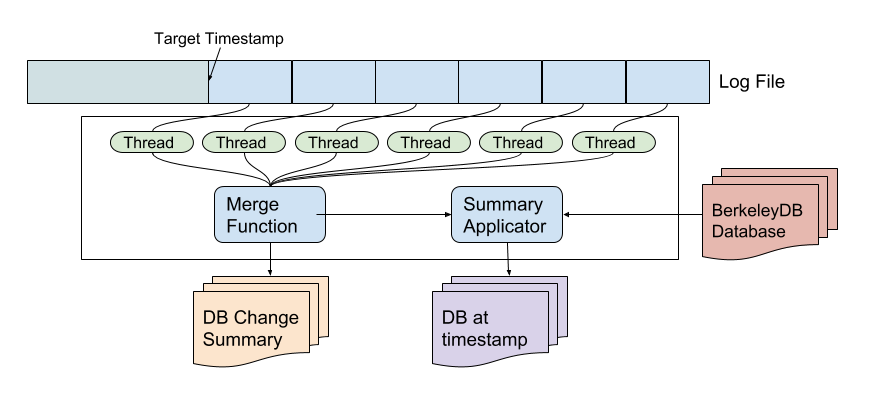
\includegraphics[height=3in]{rollbackDesgin.png}
    \caption{System Design}
    \label{fig:design1}
\end{figure*}

Different functions available to the user.

Every transaction in the database is logged just before the actual operation reads or writes to or from the disk. Logs are read and written using built in BerkeleyDB logging functions that write to a set of seperate log files. The size of each log file can be specified by the user. Each log contains a 64 bit timestamp, a transaction identifier, the type of transaction, the key being operated on, the length of the actual data being operated on, and an object storing the difference between the data before and after the transaction. This log record layout is described in figure 2.

The system supports two methods of rolling back to a user specified timestamp. Either in a linear single threaded manner, or parallelized and multithreaded. In the single threaded case the database starts at the most recent log record present in the database and walks back along the log compositing the data differences for each key as it goes. When complete it produces a single summary of everything that has changed between the present database and how it existed and the previously specified time. This summary is then applied to the present database either in place on the existing instance or on a duplicate of the database. The parallelized approach functions similarly to any other divide and conquer algorithm. It will calculate the approximate number of log records between the most recent entry and the specified rollback point. If a timestamp is to be used to specify the rollback point then the log is partitioned according to a specific time quanta. Each range of logs within a time quanta is computed by its own thread. The end result of each thread is a summary of the changes made within that time quanta. Once each thread has finished computing its summary then these summaries can be merged in a similar manner to merge-sort and a total summary of every change made to the database between the present and the specified timestamp is produced. If a copy of the database at the specified past time is desired then each summary can be applied in order to the database. In a more simple method, log sequence numbers can be used instead of timestamps in order to define roll back points and partition sizes  but the end result is very much the same as using timestamps.

In order to speed up the reconstruction process a thread could be set running in the background that would automatically produce a summary of changes for a given range of log records and store that alongside the database. Therefore whenever a roll back to a specific point in the log is desired the system only has to compute the summaries for the most recent log records and those between the specified log record and the nearest summary. This produces a situation where only two summaries must be computed instead of one for each time quanta.

\subsection{Testing Database Setup}

The database used to test the performance of the proof-of-concept implementation stored basic statistics for a set of Dungeons and Dragons characters. Each character was randomly generated using a simple C program. For each character the database stored an id, a name, a class, the character's health, whether or not the character was alive, and the character's level. In order to populate the database the user would specify a number of random transactions to perform. The transaction generator function would perform approximated an equal number of insert, retrieve, update, and delete operations.

\subsection{Implementation}
The log roll back system takes the form of a piece of basic middleware that is designed to interface with BerkeleyDB through the C API bindings and then presents itself as a library to user applications. The entirety of the program is implemented in C as it provided the right low level access and flexibility required to efficiently implement the structures that make up the core of the project.

\subsubsection{Database Context}
When a database is started it creates a context for itself. This context is used by the roll back system to define a database and its attributes. This context contains a BerkeleyDB database pointer, an environment pointer, the most recent log sequence number, the current number of keys in the database, a bit vector to keep track of unique keys, and the bit vector's length. 

\subsubsection{Unique Identifiers and Records}
One of the first challenges was keeping track of which database record a log entry is describing. To accomplish this a system of unique identifiers is used. In the system's present state the key and the identifier are the same value. The previously mentioned bit vector defined in the database's context keeps track of which unique identifiers are assigned to a database record within a given namespace. The vector rescales itself to reflect the maximum size of this namespace. This allowed for efficient re-use of identifiers as records were deleted and inserted.

The data itself takes the form of C structures. These structures are written and stored in the form of byte arrays therefore enabling easy manipulation of the records within the logging, roll back, and summary application operations.


\subsubsection{Database Functions}
A set of four functions (insert, retrieve, delete, and update) were implemented in order to provide basic functionality for the database. In general each of these functions will take in at least some of the following, a database pointer, an environment pointer, a record key, a data structure to be written, and a database context pointer. Each of these functions also handle the writing to the log whenever an operation is successful.

\begin{itemize}[noitemsep]
    \item insert(): Takes in a DB pointer, ENV pointer, a record struct, and a context pointer. Finds the first available key and writes the record struct under that key. Logs the transaction as type 0.
    \item retrieve(): Takes in a DB pointer, ENV pointer, a key, and a context pointer. Returns the record struct found at the specified key. Logs the transaction as type 1.
    \item delete(): Takes in a DB pointer, ENV pointer, a key, and a context pointer. Removes the data found the specified key and marks that key as available for use. Logs the transaction as type 2.
    \item update(): Takes in a DB pointer, ENV pointer, a key, a record struct, and a context pointer. Overwrites the data found at the specified key with the provided record struct. Logs the transaction as type 3.
\end{itemize}

\subsubsection{Log Record Management}

\begin{figure*}
    \centering
    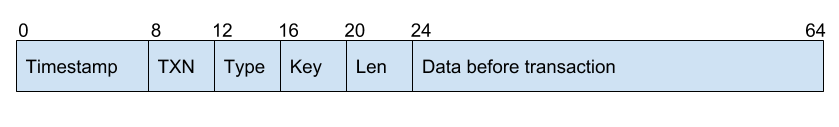
\includegraphics[height=0.75in]{LogRecordFormat.png}
    \caption{Log Record Format, the last data field in the record can vary in size based on how big a data byte array is.}
    \label{fig:design2}
\end{figure*}

As stated above the log records are created and written to a log file within each database function. The data field within each log record contains the contents of the database record before the log's corresponding operation took place. In theory this can cause the length of the log record to vary with respect to the length of the database record the log describes. Although in this implementation the data field is always 40 bytes for the sake of simplicity.

\subsubsection{Log Roll Back}

Log roll back is implemented in two different functions, linear and parallel. 
In the case of a linear roll back it will traverse a specified section of the log, which is stored in a seperate file, and compiles a summary of 
all changes made to the database. This summary takes the form of a list of byte arrays and a bitmap. 
Each byte array contains the data field of a log record while the bitmap is used to keep track of which keys were modified. In order to roll back to before an operation one must simply write this data field to the corresponding key using the standard get and put commands.

For a parallelized rollback we break up the logs between the present database configuration and the desired rollback point into a set of partitions defined by upper and lower bound log sequence numbers. 
A new thread is created for each partition and produces its own summary. Currently the summaries from each thread are not merged together but instead are applied to the database individually. One major limitation of the current implementation is that BerkeleyDB will seemingly not allow two log cursors on a single file so therefore all the threads must share. With a shared resource a locking mechanism must be implemented which then produces overhead via lock contention.


Resulting programming interface for BerkeleyDB.

\subsubsection{Underlying Database Challenges}
The initial intention was to implement a system that would produce a summary from the logs of an existing database management system such as SQLite or PostgreSQL. Out of these choices SQLite was selected as it provided more detailed technical documentation and a simpler codebase. The first challenge encountered while collecting log records for experimentation and prototyping was the fact that SQLite's log and journal files are temporary and disappear when a session is close or are cleared periodically. The second challenge was the lack of a timestamp or other easily recognizable identifying marker on each record such as a log sequence number. The lack of this feature essential to goal A would neccessitate the modification of SQLite in order to even start experimenting and collecting log information. Third was the inconvient format of having each entry in the log be a copy of a changed database page. 

It is for these reasons that BerkeleyDB was eventually chosen, albeit too late for a sophisticated implementation, for the underlying datastore and log producer. The extensive programming interface it presented allowed for much of the functionality for a roll back system to be built from the ground up as opposed to extensive and haphazard modification of an existing database system. Overall the use of BerkeleyDB as a starting point in developing the roll back system proved to be more effective as a proof of concept than the predicted path that SQLite or a more complex DBMS would have required. 

\section{Results}
In this section we evaluate the current status of the project and present performance results. All quantitative results were produced with the implemented system running on top of a BerkeleyDB key/value store configured to use a B tree. The test machine  is as follows: Ubuntu 16.04-LTS, an Intel i5-4430 (four cores at 3.2GHz), 16GB DDR3 RAM, and a 128GB Samsung SSD. 
\subsection{Implementation Status}

As of the writing of this paper goals A and B have been accomplished and goal C has been partially accomplished. The implemented system can take a database and its corresponding log and process discrete chunks of the log in a parallelized manner. When complete it outputs a summary of what exactly has changed in the database. In essence a database equivalent of the "diff" command. 

When development pivoted from the use of SQLite to the use of BerkeleyDB the original object laid out in goal C was deemed irrelevant. Although in a way it was accomplished. BerkeleyDB, while old, it still a commonly used and established piece of software and the lower level storage engine interface proved to be the right level at which to pursue an implementation of a roll back system.

Although we can say that the project has achieved the goals set at its inception the software is still far from usable. Some measurements could not be produced due to the as of yet undefined errors plaguing the system when running as a multithreaded application. Additionally the database itself cannot reliably scale beyond a size that would require more one log files as sufficiently large rollback operations would then span across said files.

%\subsection{Current Log Application Methods}

\subsection{Effects of Database Size}
\begin{figure*}
    \centering
    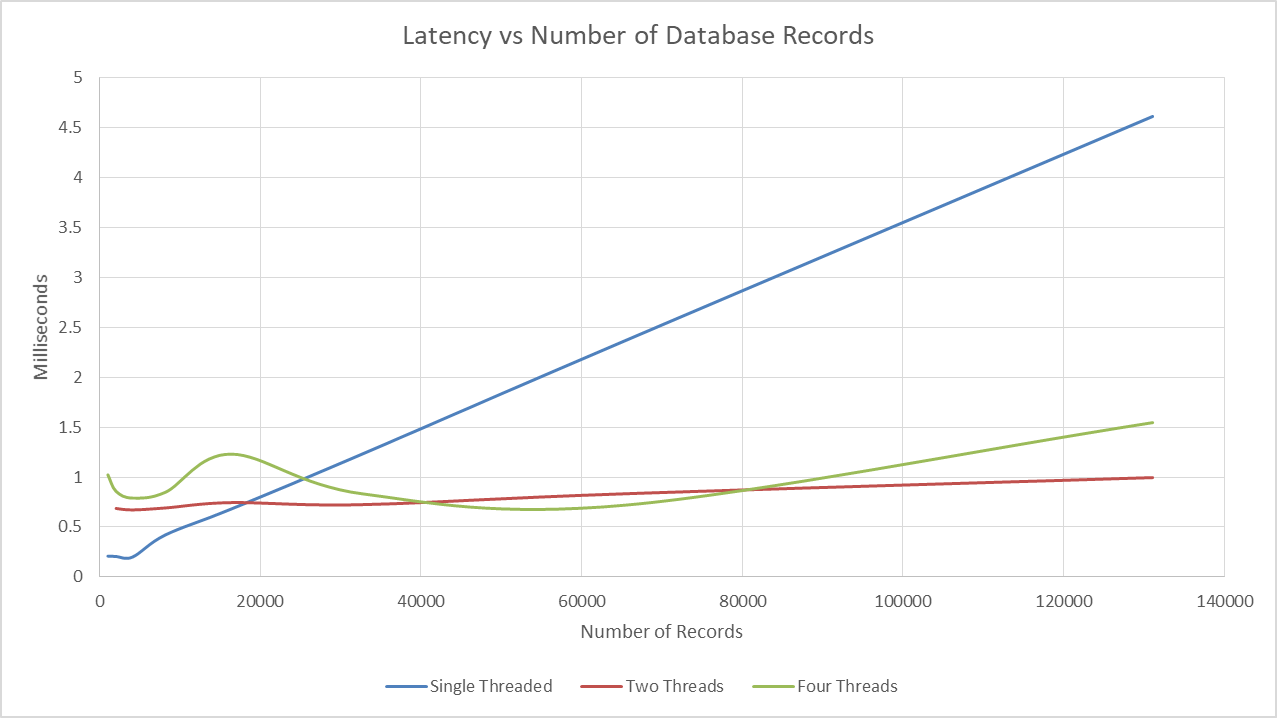
\includegraphics[height=2.5in]{latencyvsrecords.png}
    \caption{The effects of database size on summary reconstruction time. Each summary is produced by rolling back 500 log records.}
    \label{fig:DatabaseSize}
\end{figure*}

First we evaluated the latency of producing a rollback summary with respect to the size of the database. This was done on database sizes varying from 1024 records up to 131072 records, because powers of two caused the least errors during testing. Also varied was the number of threads used. Configurations of one, two, and four threads were tested. Each rollback summary consists of 500 log records. Which were divided equally in the case of multithreaded configurations. It can be observed that as the database grows in size the latency for the single threaded configuration scales linearly. In the case of both the two and four thread configurations the latency increases but at a vastly slower rate. In spite of the somewhat haphazard measurements from the four threaded configuration. Therefore for a larger database and a relatively small rollback length there is much to be gained from computing summaries in parallel.

\subsection{Effects of Rollback Length}

Next evaluated was the effect that the number of log records we would roll back by has on the amount of time needed to produce a rollback summary. For these measurements the database consisted of 65536 records with roll back lengths varying from 200 to 5000 log records. Again log records are divided equally amongst threads in multithreaded configurations.

Due to limitations posed by software errors the length of the roll backs could not be pushed to larger sizes. This is also the same reason as to why there are no results for a two thread configuration shown. We can see that up until a rollback size of 1000 records the four thread configuration performs better but once we go above that the performance begins to suffer. This is most likely due to lock contention similarly as observed by Ryan Johnson et al. in parallelized transaction processing techniques\cite{transaction}. The implemenatation tested used the BerkeleyDB log retrieval functions that relied on a log cursor, of which only one could exist without causing unrecoverable errors. Therefore each thread had to wait for a lock on the shared log cursor. Possible solutions could include multiple log files for each thread or copying each thread's partition of the log into seperate memory regions. All of which would eliminate the log cursor as a critical region. Overall with the current implementation it would be advisable to use a single threaded configuration when processing larger rollback summaries.  

\begin{figure*}
    \centering
    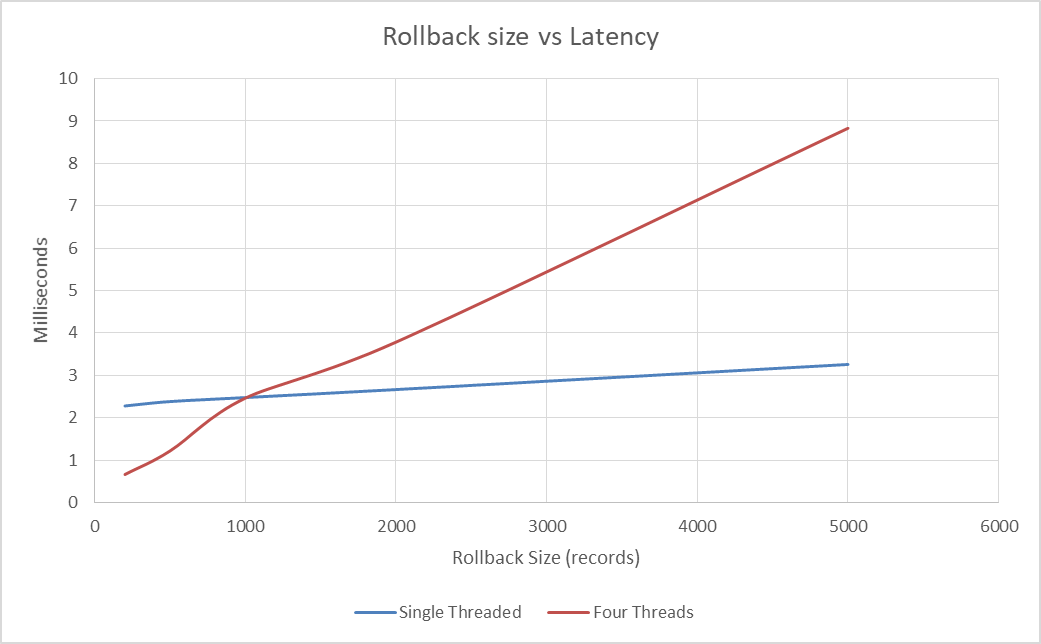
\includegraphics[height=2.5in]{sizevslatency.png}
    \caption{Effects of rollback size on summary reconstruction time. The database for each run consisted of 65536 records. Due to software errors two thread results are omitted.}
    \label{fig:RollbackSize}
\end{figure*}
\subsection{Current Limitations}
Currently the system has difficulty with larger numbers of threads, specifically more than 4. There is a significant lock contention issue when utilizing a multithreaded configuration for rollback sizes in excess of 1000 records as described earlier. The database size is likewise limited by the maximum size of the log files.

Another major limitation of this system is the log overhead. In the process of storing log records with enough information to reconstruct the database at any given time a significant amount of storage space is used. In the case of a database containing 65536 records the actual database takes up about 6.4MB but the log will easily consume 10MB worth of records for just insert operations to fill the database. Therefore it would be advisable to set a time to live (TTL) for the log records, roll them up into database summaries and store those, or some other measure to reduce the log overhead of the database.

\subsection{Future Work}
Despite the limitations of the current implementation it is evident that refinement of the presented ideas may be worth pursuing. 
Paramount to the future of this project is the stability and versatility ot its implementation. Potential future work on this system would include refactoring the codebase in order to solve the multitude of software errors that currently plague it. In the interest of determining the upper bounds on performance more deeply exploring the causes behind scalability limitations beyond four thread configurations. It would be important to rewrite the algorithm for retrieving log records from the file in such a way to reduce or eliminate lock contention and also so that it can correctly process rollbacks across multiple log files to remove the upper bound on database size. Certain features such as timestamp resolution had become lower priority in the face of the need for a minimally functional implementation. Therefore it would be advantageous to finish implementing that feature in the interest of usability. Lastly it would be beneficial to provide a system to automatically roll up log files in the background and only store the database summaries, for which the storage costs are much lower. 

\section{Conclusion}
Here we have presented a database system built on top of BerkeleyDB to allow for the parallelized roll up of logs into summaries that can possibly allow for either efficient undo operations on a database or fast rollback to a given log sequence number or timestamp. Throughout the process of implementing such a system it has been made apparent that most database systems do not possess the necessary features to easily implement the needed functionality as an add on module. Therefore it has been deemed more effective to implement the system as a form of middleware between something like a key/value store and the rest of a database management system. 

The quantitative results garnered from the initial implementation have highlighted many issues with the current implementation and a clear path forward in the systems future development. In spite of these obstacles the results are sufficient to warrant further pursuit of the project and eventual integration into a larger DBMS.
\bibliography{278}

%\end{multicols}


\end{document}
